\documentclass[twoside,11pt]{article}

% Any additional packages needed should be included after jmlr2e.
% Note that jmlr2e.sty includes epsfig, amssymb, natbib and graphicx,
% and defines many common macros, such as 'proof' and 'example'.
%
% It also sets the bibliographystyle to plainnat; for more information on
% natbib citation styles, see the natbib documentation, a copy of which
% is archived at http://www.jmlr.org/format/natbib.pdf

% Available options for package jmlr2e are:
%
%   - abbrvbib : use abbrvnat for the bibliography style
%   - nohyperref : do not load the hyperref package
%   - preprint : remove JMLR specific information from the template,
%         useful for example for posting to preprint servers.
%
% Example of using the package with custom options:
%
% \usepackage[abbrvbib, preprint]{jmlr2e}

\usepackage{jmlr2e}
\usepackage{booktabs} % for professional tables
\usepackage{amsmath,amsfonts,amssymb,mathtools}
\usepackage{algorithm}
\usepackage{algpseudocode}

% Definitions of handy macros can go here

\newcommand{\dataset}{{\cal D}}
\newcommand{\fracpartial}[2]{\frac{\partial #1}{\partial  #2}}

% Heading arguments are {volume}{year}{pages}{date submitted}{date published}{paper id}{author-full-names}

\jmlrheading{1}{2000}{1-48}{4/00}{10/00}{meila00a}{Marina Meil\u{a} and Michael I. Jordan}

% Short headings should be running head and authors last names

\ShortHeadings{Online Scalable RNNs}{Javed, Shah, Sutton, and White}
\firstpageno{1}

\newcommand{\etal}{\textit{et al}.}
\newcommand{\ie}{\textit{i}.\textit{e}., }
\newcommand{\eg}{\textit{e}.\textit{g}. }
\newcommand{\algoname}{\text{Master-User}}
\newcommand{\archi}{\text{Col-NN}}


\def\a{\alpha}
\def\b{\beta}
\def\g{\gamma}
\def\d{\delta}
\def\dd{\mbox{d}}
\def\ve{\varepsilon}
\def\e{\epsilon}
\def\n{{\bf n}}
\def\r{\rho}
\def\t{\theta}
\def\q{{\bf q}}
\def\k{{\bf k}}
\def\x{{\bf x}}
\def\y{{\bf y}}
\def\l{\ell}
\def\o{\omega}
\def\p{{\bf p}}
\def\s{\sigma}
\def\vp{\varphi}
\def\D{\Delta}
\def\E{{\bf E}}
\def\K{{\bf K}}
\def\L{{\bf L}}
\def\Pt{\tilde{P}}
\def\R{{\bf R}}
\def\S{{\bf S}}
\def\U{{\bf U}}
\def\W{{\bf W}}


\begin{document}

\title{Unbiased Scalable Online Recurrent Learning}
%\title{Recurrent Neural Network Architectures \\ for Scalable Online Learning }
%\title{Scalable Online Recurrent Learning }
%\author{\name Marina Meil\u{a} \email mmp@stat.washington.edu \\
     %  \addr Department of Statistics\\
     %  University of Washington\\
     %  Seattle, WA 98195-4322, USA
    %   \AND
    %   \name Michael I.\ Jordan \email jordan@cs.berkeley.edu \\
    %   \addr Division of Computer Science and Department of Statistics\\
    %   University of California\\
    %   Berkeley, CA 94720-1776, USA}
%
\editor{Kevin Murphy and Bernhard Sch{\"o}lkopf}

\maketitle

\begin{abstract}%   <- trailing '%' for backward compatibility of .sty file
Online scalable recurrent learning is challenging. Two popular gradient-based methods for recurrent learning are BPTT, and RTRL. BPTT looks at the complete sequence before computing gradients, and is unsuitable for online updates. RTRL can do online updates, but generally scales poorly with an increase in the number of parameters. In this paper, we propose two constraints that make RTRL scalable. We show that by either decomposing the network into independent modules, or learning a recurrent network incrementally and selectively, we can make RTRL scale linearly with the number of parameters without introducing bias, or increasing the variance of the gradient estimates. The two approaches result in different algorithms, that can be combined. We show the strengths and weaknesses of the proposed algorithms on two online prediction problems. 
\end{abstract}

\begin{keywords}
 Agent-state construction, online learning, scalable learning, recurrent learning, representation learning
\end{keywords}

\section{Introduction}
Learning by interacting with the world is a powerful framework for building systems that can autonomously achieve goals in complex worlds. A key ingredient for building autonomous systems is agent-state construction---learning a compact representation of the history of interactions that helps in predicting and controlling the future. One solution for state construction is to use differentiable recurrent neural networks (RNNs). 

State construction using RNNs requires structural credit assignment---identifying how to change network parameters to improve predictions. In RNNs, a parameter can influence  a prediction made many steps in the future. As a result, effective credit assignment requires tracking the influence of parameters on future predictions. Two popular algorithms for gradient-based structural credit assignment in recurrent neural networks are Back-propagation through time (BPTT)~(Werbos, 1988; Robinson and Fallside, 1987)  and real-time recurrent learning (RTRL)~(Williams and Zipser~1989). 

BPTT and RTRL are not suitable for online state construciton for large problems. BPTT requires storing all past activations for estimating the gradient. Additionally, it requires computation proportional to the length of the sequence seen so far. This makes BPTT unsuitable for online learning on long or never-ending streams of data. RTRL can estimate the gradient on the go, and does not require more computation as the length of the sequence grows. However, RTRL scales pooly with an increase in number of parameters of the RNN. Both BPTT and RTRL can be approximated, to make them more suitable for online learning. 

Existing approximations to gradient-based learning approximate the estimate of the gradient, but keep the function class of the network the same. These approximations either introduce bias, which can result in poor performance or even divergence, or increase the variance of the estimate, making learning extremely slow. In this work, we propose a different strategy; instead of introducing bias in the estimate of the gradient, or increase the variance of the estimate, we instead limit the function class of the RNNs in a way that allows us to compute unbiased low-variance gradient estimate in a scalable way. Limiting the function class also introduces bias, however since learning is still done using the correct gradient, our method is less susceptible to instablity in learning. 




\section{Background}
\subsection{Recurrent learning} 
\begin{equation}
y(t) = \sum_{k=0}^{d} h_k(t)w_k(t)
\end{equation}
where 
\begin{equation}
h(t) = f_{\theta(t)}\left(h(t-1), x(t)\right)
\end{equation}
here $\theta(t)$ are the parameters of the RNN at time $t$, whereas $f_\theta$ is a function that represents the RNN. Given this notation, we can write the gradient of a prediction $y(t)$ w.r.t the parameters $\theta$ as
\begin{equation}
\begin{aligned}
\frac{\partial{y(t)}}{\partial{\theta}} & = \frac{\partial{y(t)}}{\partial{h(t)}}\frac{\partial{h(t)}}{\partial{\theta}}   \\
\end{aligned}
\end{equation}
We can expand the second term as: 
\begin{equation}
\frac{\partial{h(t)}}{\partial{\theta}} =  \frac{\partial{h(t)}}{\partial{\theta(t)}} + \frac{\partial{h(t)}}{\partial{h(t-1)}} \frac{\partial{h(t-1)}}{\partial{\theta}}
\label{expansion}
\end{equation}
to get
\begin{equation}
\frac{\partial{y(t)}}{\partial{\theta}}  = \frac{\partial{y(t)}}{\partial{h(t)}}\left(\frac{\partial{h(t)}}{\partial{\theta(t)}} + \frac{\partial{h(t)}}{\partial{h(t-1)}} \frac{\partial{h(t-1)}}{\partial{\theta}}  \right) 
\label{expanded}
\end{equation}
Note that we can use equation~\ref{expansion} to recursively expand equation~\ref{expanded}, until we can get rid of $\partial \theta$ term.  
BPTT estimates the gradient of $y(t)$ by repeatedly using equation~\ref{expansion}. 

BPTT extends the back-propagation algorithm for feed-forward networks---independently proposed by Werbos~(1974) and Rumelhart~\etal~(1986)---to RNNs by storing network activations from prior steps, and repeatedly applying the chain-rule starting from the output of the network and ending at the activations at the beginning of the sequence. More precisely, we can write the gradient of a prediction $y(t)$ w.r.t the parameters $\theta$ as:

where $h(t)$ is the internal state of the network at time $t$. Then, BPTT comput
BPTT is unsuitable for online learning as it requires memory proportional to the length of the sequence. Moreover, it delays gradient computation until the end of the sequence. For online learning, this sequence can be arbitrarily long or never-ending.
\begin{algorithm}
\caption{Back-propagation through time}\label{alg:cap}
\begin{algorithmic}
	\Require $x_1, x_2, x_3, x_4, \cdots, x_n$
	\Require $h_0$
	\Require $\theta_1$
	\State $X \gets x$
	\State $N \gets n$
	\For{$t$ in $1, 2, 3, \cdots, n$}
		\State $h_t = f_{\theta_t}(h_{t-1}, x_t)$
	\EndFor
	\State $y_t = \sum_{k=0}^{d} w_k h_k^t$
	\State grad = 0
	\For{$t$ in $n, n-1, \cdots, 1$}
	\State 
	\EndFor
	 
\end{algorithmic}
\end{algorithm}


\begin{algorithm}
	\caption{Real-time recurrent learning}\label{alg:cap}
	\begin{algorithmic}
		\Require $n \geq 0$
	\end{algorithmic}
\end{algorithm}



% The dependence of BPTT on storing activations from past hinders its application to online learning. Additionally, the computation in BPTT is not spread uniformly across time --- the learner accumulates activations for a sequence in the memory and delays the computation of the gradients until the end. This is incompatible with the goal of real-time learning --- the ability to incorporate feedback from the environment quickly for correcting mistakes. 


RTRL---an alternative to BPTT---was proposed by Williams and Zipser~(1989). RTRL relies on forward-mode differentiation---using chain-rule to compute gradients in the direction of time---to compute gradients recursively. Unlike BPTT, RTRL does not delay gradient-computation until the final step. The memory requirement of RTRL also does not depend on the sequence length. As a result, it is more suitable for real-time online learning. Unfortunately, RTRL requires maintaining the Jacobian $\frac{\partial h(t)}{\partial \theta}$ at every step, which requires $O(|h||\theta|)$ memory, where $|h|$ is the size of state of the network and $|\theta|$ is the number of total parameters. The Jacobian is recursively updated by applying chain rule as:  
$$\frac{\partial h(t+1)}{\partial \theta} =\frac{\partial h(t+1)}{\partial \theta(t+1)} +  \frac{\partial h(t+1)}{\partial h(t)}\frac{\partial h(t)}{\partial \theta}, $$ 
which requires  $O(|h|^2|\theta|)$ operations and scales poorly to large networks.

% For a more thorough explanation of the memory and time complexity of recurrent state-learning and meta-learning methods using RTRL, see Appendix A. 



A promising direction to scale gradient-based credit-assignment to large networks is to approximate the gradient. Elman~(1990) proposed to ignore the influence of parameters on future predictions completely for training RNNs. This resulted in a scalable but biased algorithm. Williams and Peng~(1990) proposed a more general algorithm called Truncated BPTT (T-BPTT). T-BPTT tracks the influence of all parameters on predictions made up to $k$ steps in the future. T-BPTT limits the BPTT computation to last $k$ steps, and works well for a range of problems~(Mikolov~\etal, 2009, 2010; Sutskever, 2013 and Kapturowski~\etal, 2018). Its main limitation is that the resultant gradient is blind to long-range dependencies. Mujika~\etal~(2018) showed that on a simple copy task, T-BPTT failed to learn dependencies beyond the truncation window. Tallec~\etal~(2017) demonstrated T-BPTT can even diverge when a parameter has a negative long-term effect on a target and a positive short-term effect. 

\begin{figure*}
	\centering
	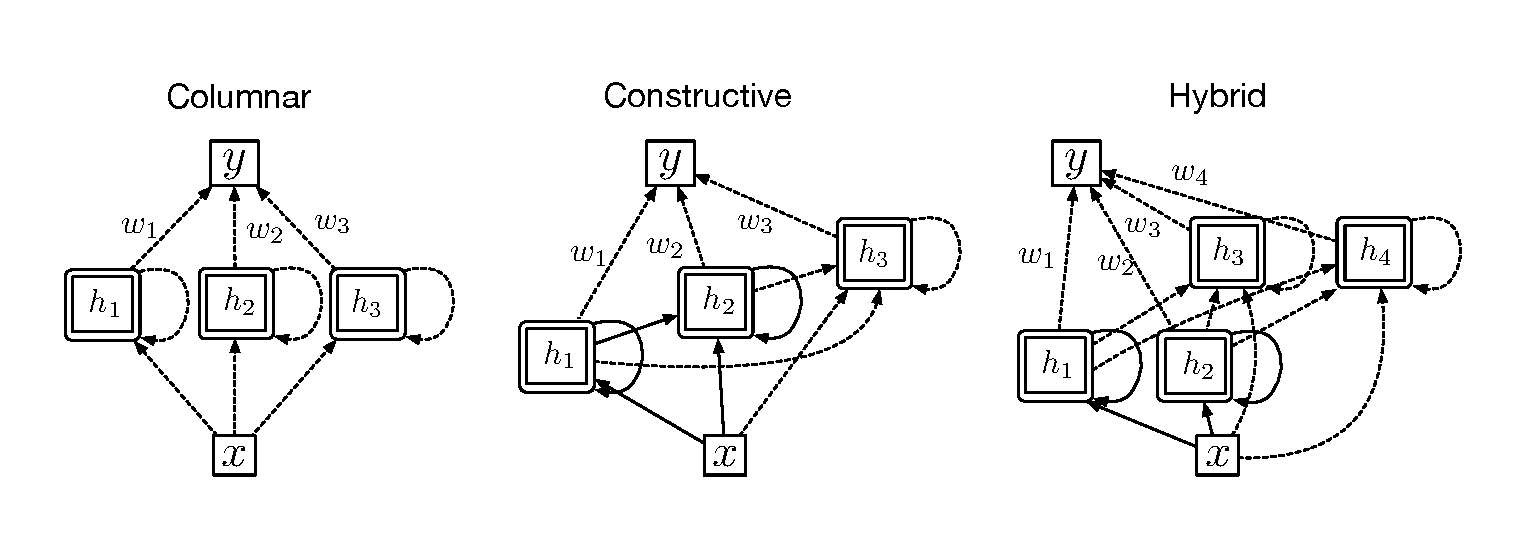
\includegraphics[width=0.95\textwidth]{figures/three_types}
	\caption{TODO: Make the caption concise. Three structures of recurrent neural networks that can be trained without truncation. Recurent networks with a columnar structure can be trained end-to-end using gradients without any truncation, only requiring $O(n)$ operations and memory per step. However, columnar networks do not have hierarchical recurrent features---recurrent features made out of other recurrent features. Constructive networks have hierarchical recurrent features, however must be trained incrementally to prevent bias. Incremental learning is achieved by initializing all $w_i$ to zero, and learning $h_1$, $h_2$, and $h_3$ in order. Finally, columnar and constructive networks can be combined to get a hybrid network. The pairs $(h_1, h_2)$ and $(h_3, h_4)$ do not depend on each other, and can learn in parallel. Hoever, $(h_3, h_4)$ must be learned after $(h_1, h_2)$ have been learned and fixed.}
\end{figure*}

RTRL can also be approximated to reduce its computational overhead. Ollivier~\etal~(2015) and Tallec~\etal~(2017) proposed NoBacktrack and UORO. Both of these algorithms provide stochastic unbiased estimates of the gradient and scale well. However, their estimates have high variance and require extremely small step sizes for effective learning. Cooijmans, Martens~(2019) and Menick~\etal~(2021) showed that, for practical problems, UORO does not perform well compared to other biased approximations due to the high variance in its gradient estimates . Menick~\etal~(2021) proposed an approximation to RTRL called SnAp-$k$. SnAp-$k$ tracks the influence of a parameter on a state only if the parameter can influence the state within $k$ steps. It first identifies parameters whose influence on a state is zero for $k$ steps and then assumes the future influence to be zero as well. For the remaining parameters, it tracks their influence on all future predictions. The bias introduced by SnAp-k is fundamentally different than the bias introduced by T-BPTT. SnAp-1 can be computationally efficient but introduces significant bias. SnAp-$k$ for $k>1$ reduces bias but can be as expensive as RTRL for dense RNNs.  Menick~\etal~(2021) further proposed using sparse connections as a way to make SnAp more scalable. Connection sparsity reduces the number of parameters that can influence a state within $k$ steps. 

Among all the approximations, SnAp-1 is the only method that scales linearly with number of parameters, is capable of learning long-term dependencies, and 

\subsection{General value functions and }
\section{Problem Formulation} 
We formulate the problem as predicting the discounted some of a cumulant from an online stream of data. More formally, the agent sees a feature vector $x(t)\in \mathcal{R}^d$ at timestep $t$ and predicts the discounted sum of a cumulant $y_t$ given by: 
\begin{equation}
\begin{aligned}
V(S_t) & = \mathbb{E}[G_t | S_t] \\
& = \mathbb{E}[\sum_{k = 0}^{\infty} \gamma^k y(k)]
\end{aligned}
\end{equation}
Our problem formulation can be used to represent temporal predictions, such as policy evaluation and general value functions. Additionally, by setting $\gamma = 0$, our problem formulation can represent classifcal supervised recurrent learning benchmarks. The goal of the agent is to minimize the mean squared error between the prediction $\hat{V}(x_{1:t})$ and $V(S)$. Note that for all our experiments, the data generation policy $\pi$ is fixed and can be ignored. 

\section{Divergence for truncated-backprop and Snap-1}
Because truncated backprop and Snap-1 use biased estimates of the gradients for learning updates, they can cause the prediction error and parameters to diverge under pathological cases. We present examples of divergence for both truncated-bptt and SnAp-1. In real-world case, such divergence happens rarely, if ever. However the examples still serve a useful pedagogical role, to clarify the limitation of the two algorithms. 

For truncated backprop, we use a simple recurrent network with one hidden unit, one feature, and one prediction. The recurrence is defined as adding the value of the last hidden state to the current state. We fix the weight for the recurrent connection and the outgoing connection, and learn only the incoming weight. The optimal solution is $w_{in} = -10$. We let the recurrent network learn for a thousand steps using a step size of $10^{-3}$ and show the behavior pf th elearning algorithm in Figure~. Note that the learning 
\section{Proposed methods} 
We propose imposing a specific structure on either the connections of the recurrent network, or the learning algorithms, to achieve scalable learning without truncation. We propose columnar networks to ac

\section{Empirical evaluation} 

\begin{figure*}
	\centering
	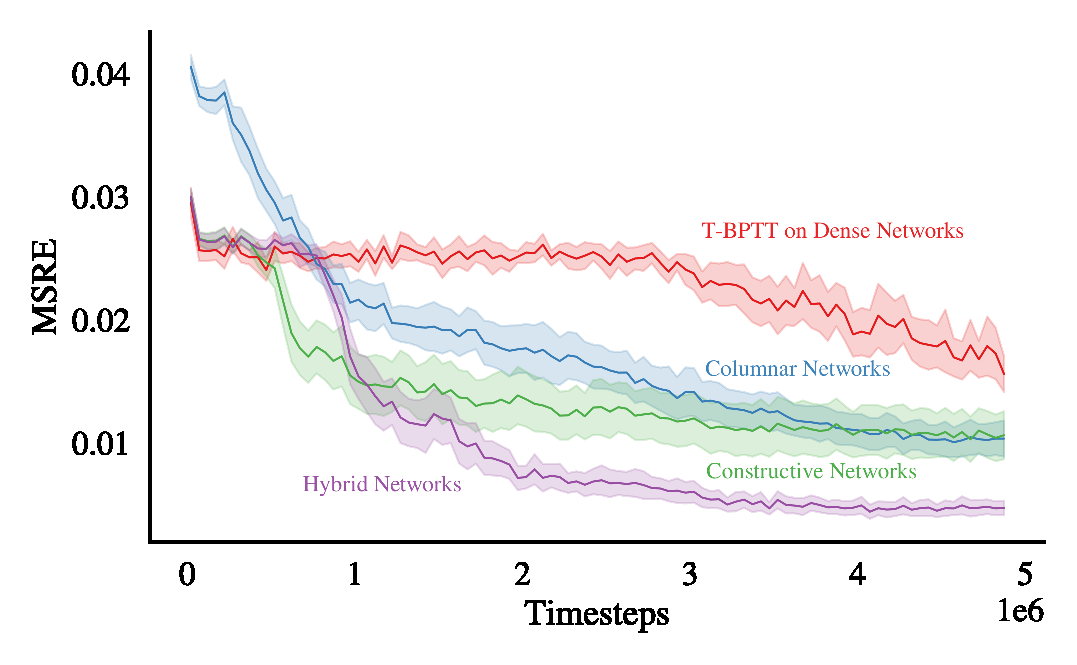
\includegraphics[width=0.75\textwidth]{figures/plt_animal.eps}
	\caption{TODO: T-BPTT is only 15 runs while the remaining curves are 30 runs. }
\end{figure*}
We first evaluate the performance of the proposed methods, and baselines, on a set of 
\section{Temporally symmetric hierarchical recurrent learning using generate and test}  
The primary limitation of the constructive and hybrid approaches is that they are not suitable for continual learning. Once a feature is frozen, it never changes, even if the environment does. In the constructive case, the agent can, at best, continually update one recurrent feature. In the hybrid case, the agent can update $k$ recurrent units added last. Inability to update all features after a certain number of time steps  make the agent lose the ability to  modify its feature representation. In a sense, the agent becomes a linear learner. 

We can address this limitation by identifying features that are no longer useful, and pruning them. These pruned features can then be replaced with newly constructed features. Similar ideas have been proposed in literature under the term generate and test. 

To effectively combine our method with generate and test, we need to answer two questions---(1) how useless features are identified, and (2) how new features replace them. It is unclear what an ideal algorithm to answer these two questions are. In this work, we limit ourselves to the simple algorithms for both questions. The goal here is to present one temporally symmetric version of the hybrid approach, and not to figure out the best temporally symmetric version. 

To identify useless features, we simply look at how much a feature contributes to its outgoing connection, and use the sum of contribution to all outgoing connections as the utility of the feature. The contribution of a feature to an outgoing connection is defined as the 

%  SnAp, combined with sparsity, is a promising research direction.

%Menick~\etal~(2021) showed that for highly sparse networks, SnAp-$k$ reduces the computational requirement of RTRL by over 95\% while keeping bias in check. One limitation of their work is that they do not provide a scalable method to identify parameters that would not influence a state within $k$ steps. Instead, they run the RNN for $k$ steps and look at the full Jacobian $\frac{\partial h(t)}{\partial \theta}$ to determine these parameters. For large networks, computing this Jacobian even once is not possible. Moreover, because they induce sparsity randomly in their networks, the resultant sparsity in the Jacobian is not structured and is not amenable to efficiency gains using existing hardware. Finally, SnAp does not scale well when used in conjunction with deep feature extractors. If internal states operate on a shared representation computed with a deep network with parameters $\theta$, even SnAp-1 could require $O(|\theta||h|)$ memory and $O(|\theta||h|^2)$ operations per-step. Our goal is to design an algorithm that requires $O(|\theta|)$ memory and operations.




% Acknowledgements should go at the end, before appendices and references

\acks{We would like to acknowledge support for this project
from the National Science Foundation (NSF grant IIS-9988642)
and the Multidisciplinary Research Program of the Department
of Defense (MURI N00014-00-1-0637). }

% Manual newpage inserted to improve layout of sample file - not
% needed in general before appendices/bibliography.

\newpage

\appendix
\section*{Appendix A.}

\section{Forward-mode gradient computation of an LSTM cell }

Here we derive the update equations for recursively computing the gradients of a single LSTM based recurrent column. Each column has a single hidden unit. Because all columns are identical, the same update equations can be used to learn the complete Columnar Network.  The state of an LSTM column is updated using following equations: 
% \begin{equation}
% \label{lstm}
\begin{align}
i(t) &= \sigma( W_{i}^T x_k(t) + u_{i} h(t-1) + b_i) \label{i} \\
f(t) &= \sigma( W_{f}^T x_k(t) + u_{f} h(t-1) + b_f) \label{f} \\
o(t) &= \sigma( W_{o}^T x_k(t) + u_{o} h(t-1) + b_o) \label{o} \\
g(t) &= \phi( W_{g}^T x_k(t) + u_{g} h(t-1) + b_g) \label{g} \\
c(t) &= f(t)  c(t-1) + i(t) g(t) \label{c} \\
h(t) &= o(t)  \phi(c(t)) \label{state_update}
\end{align}
% \end{equation}
where $\sigma$ and $\phi$ are the sigmoid and tanh activation functions, $h(t)$ is the state of the column at time $t$ and $ W_{i}^T x_k(t) = \sum_{k=1}^m W_{i_k} x_k(t)$. The derivative of $\sigma(x)$ and $\phi(x)$ w.r.t to $x$ are $\sigma(x)(1-\sigma(x))$ and $(1-\phi^2(x))$ respectively.

Let the length of input vector $x$ be $m$. Then, $W_{i}, W_{f}, W_{o}$ and $W_{g}$ are vectors of length $m$ whereas $u_i, b_i, u_f, b_f, u_o, b_o, u_g$ and $b_g$ are scalars. We want to compute gradient of $h(t)$ with respect to all the parameters. We derive the update equations for $\frac{\partial h(t)}{\partial W_{i}} ,\frac{\partial h(t)}{\partial u_{i}}, $$\frac{\partial h(t)}{\partial b_{i}}, \frac{\partial h(t)}{\partial W_{f}} $$,\frac{\partial h(t)}{\partial u_{f}}, \frac{\partial h(t)}{\partial b_{f}}, $$\frac{\partial h(t)}{\partial W_{o}} ,\frac{\partial h(t)}{\partial u_{o}},$$ \frac{\partial h(t)}{\partial b_{o}}, \frac{\partial h(t)}{\partial W_{g}} ,\frac{\partial h(t)}{\partial u_{g}},$ and $\frac{\partial h(t)}{\partial b_{g}}$ in the following sections. 

\subsection{$\frac{\partial h(t)}{\partial W_{i}}$}

$W_i = (W_{i_1}, W_{i_2}, \cdots, W_{i_m})$ is a vector of length $m$. Since all elements of $W_i$ are symmetric, we show gradient derivation for $W_{i_j}$ without loss of generality. Let
% \begin{equation}
\begin{align}
TH_{W_{i_j}}(t)  & \vcentcolon = \frac{\partial h(t)}{\partial W_{i_j}}  && \textit{(By definition)} \label{def1} \\
TH_{W_{i_j}}(0)  & \vcentcolon = 0  && \textit{(By definition)} \label{def2} \\
TC_{W_{i_j}}(t)  & \vcentcolon = \frac{\partial c(t)}{\partial W_{i_j}}  && \textit{(By definition)} \label{def3} \\
TC_{W_{i_j}}(0)  & \vcentcolon = 0  && \textit{(By definition)}  \label{def4}
% %   & = (1-z^k(t)) T_{w_{z}}^{ijk}(t-1) + z^k(t) \frac{\partial}{\partial W^{ij}_z}\left (  z^k(t)  \hat{h}^k(t) \right )  && \textit{Using definition 5}\\
% %   & = (1-z^k(t)) T_{w_{z}}^{ijk}(t-1) + z^k(t) \frac{\partial \hat{h}^k(t)}{\partial W^{ij}_z} + \hat{h}^k(t) \frac{\partial z^k(t)}{\partial W^{ij}_z}  && \textit{test} \textit{Applying chain rule}
\end{align}
% \end{equation}
Then:
% \begin{equation}
\begin{align*}
TH_{W_{i_j}}(t) & = \frac{\partial}{\partial W_{i_j}} \left ( o(t) \phi(c(t)) \right ) && \textit{From equation \ref{state_update} and definition \ref{def1}} \\
& = o(t) \frac{\partial \phi(c(t))}{\partial W_{i_j}}  + \phi(c(t)) \frac{\partial o(t)}{\partial W_{i_j}}   && \textit{Product rule of differentiation} \\
&= o(t) (1-\phi^{2}(c(t))) \frac{\partial c(t)}{\partial W_{i_j}}  + \phi(c(t)) \frac{\partial o(t)}{\partial W_{i_j}}   && \textit{Derivative of $\phi(x)$ is (1-$\phi^2(x))$}\\ 
&= o(t) (1-\phi^{2}(c(t))) TC_{W_{i_j}}(t)  + \phi(c(t)) \frac{\partial o(t)}{\partial W_{i_j}}   && \textit{From definition \ref{def3}}\\ 
\frac{\partial o(t)}{\partial W_{i_j}} &=  \frac{\partial}{\partial W_{i_j}} \sigma(W_{o}^T x(t) + u_{o} h(t-1) + b_o) && \textit{From equation \ref{o}}\\
&= \sigma(y)(1-\sigma(y))u_o TH_{W_{i_j}}(t-1) && \textit{Where $y$ equals $W_{o}^T x(t) + u_{o} h(t-1) + b_o$} \\
TC_{W_{i_j}}(t) &=  \frac{\partial c(t)}{\partial W_{i_j}} && \textit{From definition \ref{def3}} \\ 
&=  \frac{\partial}{\partial W_{i_j}} (f(t)  c(t-1) + i(t) g(t))  && \textit{From equation \ref{c}} \\
&= f(t) TC_{W_{i_j}}(t-1) + c(t-1)\frac{\partial f(t)}{ \partial W_{i_j}} + \frac{\partial}{\partial W_{i_j}} ( i(t) g(t) )   && \textit{Product rule and definition \ref{def3}}\\
&= f(t) TC_{W_{i_j}}(t-1) + c(t-1)\frac{\partial f(t)}{ \partial W_{i_j}} + i(t)\frac{\partial g(t) }{\partial W_{i_j}}  + g(t)\frac{\partial i(t) }{\partial W_{i_j}}  && \textit{Product rule} 
% %   & = (1-z^k(t)) T_{w_{z}}^{ijk}(t-1) + z^k(t) \frac{\partial}{\partial W^{ij}_z}\left (  z^k(t)  \hat{h}^k(t) \right )  && \textit{Using definition 5}\\
% %   & = (1-z^k(t)) T_{w_{z}}^{ijk}(t-1) + z^k(t) \frac{\partial \hat{h}^k(t)}{\partial W^{ij}_z} + \hat{h}^k(t) \frac{\partial z^k(t)}{\partial W^{ij}_z}  && \textit{test} \textit{Applying chain rule}
\end{align*}


% \end{equation}

Where gradient of $g(t)$  w.r.t $W_{i_j}$ is:
% \begin{equation}
\begin{align*}
\frac{\partial g(t)}{\partial W_{i_j}} &=  \frac{\partial}{\partial W_{i_j}} \phi(W_{g}^T x(t) + u_{g} h(t-1) + b_g) && \textit{From equation \ref{g}} \\
&= (1-\phi^2(y))u_g TH_{W_{i_j}}(t-1) && \textit{Where $y$ equals $W_{g}^T x(t) + u_{g} h(t-1) + b_g$} \\
\end{align*}
% \end{equation}
, gradient of $f(t)$  w.r.t $W_{i_j}$ is:
% \begin{equation}
\begin{align*}
\frac{\partial f(t)}{\partial W_{i_j}} &=  \frac{\partial}{\partial W_{i_j}} \sigma(W_{f}^T x(t) + u_{f} h(t-1) + b_f) && \textit{From equation \ref{f}} \\
&= \sigma(y)(1-\sigma(y))u_f TH_{W_{i_j}}(t-1) && \textit{Where $y$ equals $W_{f}^T x(t) + u_{f} h(t-1) + b_f$} \\
\end{align*}
% \end{equation}
and gradient of $i(t)$ w.r.t $W_{i_j}$ is:
% \begin{equation}
\begin{align*}
\frac{\partial i(t)}{\partial W_{i_j}} &=  \frac{\partial}{\partial W_{i_j}} \sigma(W_{i}^T x(t) + u_{i} h(t-1) + i_f) && \textit{From equation \ref{i}} \\
&= \sigma(y)(1-\sigma(y)) \left (x_j(t)+ u_i TH_{W_{i_j}}(t-1) \right )&& \textit{Where $y$ equals $W_{i}^T x(t) + u_{i} h(t-1) + b_i$} \\
\end{align*}
% \end{equation}
The derivation shows that using two traces per parameter of $W_i$, it is possible to compute the gradient of $h(t)$ w.r.t $W_i$ recursively. We provide the derivations for parameters $u_i$ and $b_i$ below. We skip the step-by-step derivations for the remaining parameters as they are similar. 

\subsection{$\frac{\partial h(t)}{\partial u_i}$}

% \begin{equation}
\begin{align}
TH_{u_{i}}(t)  & \vcentcolon = \frac{\partial h(t)}{\partial u_i}  && \textit{(By definition)}  \label{thu}\\
TH_{u_{i}}(0)  & \vcentcolon = 0  && \textit{(By definition)}  \\
TC_{u_{i}}(t)  & \vcentcolon = \frac{\partial c(t)}{\partial u_i}  && \textit{(By definition)}  \label{tcu} \\
TC_{u_{i}}(0)  & \vcentcolon = 0  && \textit{(By definition)} 
\end{align}
% \end{equation}

% \begin{equation}
\begin{align*}
TH_{u_i}(t) & = \frac{\partial}{\partial u_i} \left ( o(t) \phi(c(t)) \right ) && \textit{From equation \ref{state_update}} \\
& = o(t) \frac{\partial \phi(c(t))}{\partial u_i}  + \phi(c(t)) \frac{\partial o(t)}{\partial u_i}   && \textit{Product rule} \\
&= o(t) (1-\phi^{2}(c(t))) \frac{\partial c(t)}{\partial u_i}  + \phi(c(t)) \frac{\partial o(t)}{\partial u_i}   && \textit{Derivative of $\phi(x)$ is $1-\phi^2(x)$} \\
&= o(t) (1-\phi^{2}(c(t))) TC_{u_{i}}(t)  + \phi(c(t)) \frac{\partial o(t)}{\partial u_i}   && \textit{Using definition \ref{tcu}} \\
\frac{\partial o(t)}{\partial u_i} &=  \frac{\partial}{\partial u_i} \sigma(W_{o}^T x(t) + u_{o} h(t-1) + b_o) && \textit{Using equations \ref{o}}\\
&= \sigma(x)(1-\sigma(x))u_o TH_{u_i}(t-1) && \textit{Where $x$ equal $W_{o}^T x(t) + u_{o} h(t-1) + b_o$} \\
TC_{u_i}(t) &=  \frac{\partial c(t)}{\partial u_i} && \textit{Definition \ref{tcu}} \\ 
&=  \frac{\partial}{\partial u_i} (f(t)  c(t-1) + i(t) g(t))  && \textit{From equation \ref{state_update}} \\
&= f(t) TC_{u_i}(t-1) + c(t-1)\frac{\partial f(t)}{ \partial u_i} + \frac{\partial}{\partial u_i} \left ( i(t) g(t) ) \right )  && \textit{Product rule}\\
&= f(t) TC_{u_i}(t-1) + c(t-1)\frac{\partial f(t)}{ \partial u_i} + i(t)\frac{\partial g(t) }{\partial u_i}  + g(t)\frac{\partial i(t) }{\partial u_i}  && \textit{Product rule} 
% %   & = (1-z^k(t)) T_{w_{z}}^{ijk}(t-1) + z^k(t) \frac{\partial}{\partial W^{ij}_z}\left (  z^k(t)  \hat{h}^k(t) \right )  && \textit{Using definition 5}\\
% %   & = (1-z^k(t)) T_{w_{z}}^{ijk}(t-1) + z^k(t) \frac{\partial \hat{h}^k(t)}{\partial W^{ij}_z} + \hat{h}^k(t) \frac{\partial z^k(t)}{\partial W^{ij}_z}  && \textit{test} \textit{Applying chain rule}
\end{align*}
% \end{equation}
Gradient of  $g(t)$  w.r.t  $u_i$ is:
% \begin{equation}
\begin{align*}
\frac{\partial g(t)}{\partial u_i} &=  \frac{\partial}{\partial u_i} \phi(W_{g}^T x(t) + u_{g} h(t-1) + b_g) && \textit{From equations \ref{state_update}} \\
&= (1-\phi^2(y))u_g TH_{u_i}(t-1) && \textit{Where $y$ equals $W_{g}^T x(t) + u_{g} h(t-1) + b_g$} \\
\end{align*}
% \end{equation}
, gradient of $f(t)$  w.r.t $u_i$ is:
% \begin{equation}
\begin{align*}
\frac{\partial f(t)}{\partial u_i} &=  \frac{\partial}{\partial u_i} \sigma(W_{f}^T x(t) + u_{f} h(t-1) + b_f) && \textit{From equations 1} \\
&= \sigma(y)(1-\sigma(y))u_f TH_{u_i}(t-1) && \textit{Where $y$ equals $W_{f}^T x(t) + u_{f} h(t-1) + b_f$} \\
\end{align*}
% \end{equation}

and the gradient of $i(t)$  w.r.t $u_i$ is
% \begin{equation}
\begin{align*}
\frac{\partial i(t)}{\partial u_i} &=  \frac{\partial}{\partial u_i} \sigma(W_{i}^T x(t) + u_{i} h(t-1) + b_i) && \textit{Using equations 1} \\
&= \sigma(y)(1-\sigma(y)) \left (h(t-1)+ u_i TH_{u_{i}}(t-1) \right )&& \textit{Where $y$ equals $W_{i}^T x(t) + u_{i} h(t-1) + b_i$} \\
\end{align*}
% \end{equation}

\subsection{$\frac{\partial h(t)}{\partial b_i}$}

% \begin{equation}
\begin{align}
TH_{b_i}(t)  & \vcentcolon = \frac{\partial h(t)}{\partial b_i}  && \textit{(By definition)}  \label{thb}\\
TH_{b_i}(0)  & \vcentcolon = 0  && \textit{(By definition)}  \\
TC_{b_i}(t)  & \vcentcolon = \frac{\partial c(t)}{\partial b_i}  && \textit{(By definition)}  \label{tcb}\\
TC_{b_i}(0)  & \vcentcolon = 0  && \textit{(By definition)} 
\end{align}
% \end{equation}

% \begin{equation}
\begin{align*}
TH_{b_i}(t) & = \frac{\partial}{\partial b_i} \left ( o(t) \phi(c(t)) \right ) && \textit{From equation \ref{state_update}} \\
& = o(t) \frac{\partial \phi(c(t))}{\partial b_i}  + \phi(c(t)) \frac{\partial o(t)}{\partial b_i}   && \textit{Product rule} \\
&= o(t) (1-\phi^{2}(c(t))) \frac{\partial c(t)}{\partial b_i}  + \phi(c(t)) \frac{\partial o(t)}{\partial b_i}   && \textit{Derivative of of $\phi(x)$ is $1-\phi^2(x)$}\\ 
&= o(t) (1-\phi^{2}(c(t))) TC_{b_i}(t)  + \phi(c(t)) \frac{\partial o(t)}{\partial b_i}   && \textit{From definition \ref{tcb} }\\ 
\frac{\partial o(t)}{\partial b_i} &=  \frac{\partial}{\partial b_i} \sigma(W_{o}^T x(t) + u_{o} h(t-1) + b_o) && \textit{From equations \ref{o}}\\
&= \sigma(y)(1-\sigma(y))u_o TH_{b_i}(t-1) && \textit{Where $y$ equal $W_{o}^T x(t) + u_{o} h(t-1) + b_o$} \\
TC_{b_i}(t) &=  \frac{\partial c(t)}{\partial b_i} && \textit{From definition \ref{tcb}} \\ 
&=  \frac{\partial}{\partial b_i} (f(t)  c(t-1) + i(t) g(t))  && \textit{From equation \ref{c}} \\
&= f(t) TC_{b_i}(t-1) + c(t-1)\frac{\partial f(t)}{ \partial b_i} + \frac{\partial}{\partial b_i}  i(t) g(t)   && \textit{Product rule}\\
&= f(t) TC_{b_i}(t-1) + c(t-1)\frac{\partial f(t)}{ \partial b_i} + i(t)\frac{\partial g(t) }{\partial b_i}  + g(t)\frac{\partial i(t) }{\partial b_i}  && \textit{Product rule} 
% %   & = (1-z^k(t)) T_{w_{z}}^{ijk}(t-1) + z^k(t) \frac{\partial}{\partial W^{ij}_z}\left (  z^k(t)  \hat{h}^k(t) \right )  && \textit{Using definition 5}\\
% %   & = (1-z^k(t)) T_{w_{z}}^{ijk}(t-1) + z^k(t) \frac{\partial \hat{h}^k(t)}{\partial W^{ij}_z} + \hat{h}^k(t) \frac{\partial z^k(t)}{\partial W^{ij}_z}  && \textit{test} \textit{Applying chain rule}
\end{align*}
% \end{equation}
Where gadient of  $g(t)$  w.r.t $b_i$ is:
\begin{align*}
\frac{\partial g(t)}{\partial b_i} &=  \frac{\partial}{\partial b_i} \phi(W_{g}^T x(t) + u_{g} h(t-1) + b_g) && \textit{From equation \ref{g}} \\
&= (1-\phi^2(y))u_g TH_{b_i}(t-1) && \textit{Where $y$ equal $W_{g}^T x(t) + u_{g} h(t-1) + b_g$} \\
\end{align*}

, gradient of $f(t)$  w.r.t $b_i$ is:
% \begin{equation}
\begin{align*}
\frac{\partial f(t)}{\partial b_i} &=  \frac{\partial}{\partial b_i} \sigma(W_{f}^T x(t) + u_{f} h(t-1) + b_f) && \textit{From equation \ref{f}} \\
&= \sigma(y)(1-\sigma(y))u_f TH_{b_i}(t-1) && \textit{Where $y$ equal $W_{f}^T x(t) + u_{f} h(t-1) + b_f$} \\
\end{align*}
% \end{equation}

and gradient of $i(t)$  w.r.t $b_i$ is:
% \begin{equation}
\begin{align*}
\frac{\partial i(t)}{\partial b_i} &=  \frac{\partial}{\partial b_i} \sigma(W_{i}^T x(t) + u_i h(t-1) + b_i) && \textit{From equation \ref{i}} \\
&= \sigma(y)(1-\sigma(y)) \left (u_i TH_{b_i}(t-1) + 1 \right )&& \textit{Where $y$ equal $W_{i}^T x(t) + b_i h(t-1) + b_i$} \\
\end{align*}
% \end{equation}


\subsection{$\frac{\partial h(t)}{\partial W_{f_j}}$}
The derivations for the remaining parameters is analogous to what previous derivations. The final equations are as follows.
\begin{equation}
\begin{aligned}
\frac{\partial g(t)}{\partial W_{f_j}} &=  (1-\phi^2(y))(u_g TH_{W_{f_j}}(t-1))  \\
\frac{\partial f(t)}{\partial W_{f_j}} &=  \sigma(y)(1-\sigma(y))( x_j + u_f TH_{W_{f_j}}(t-1)) \\
\frac{\partial i(t)}{\partial W_{f_j}}  &= \sigma(y)(1-\sigma(y))( u_i TH_{W_{f_j}}(t-1))  \\
\frac{\partial o(t)}{\partial W_{f_j}} &=  \sigma(y)(1-\sigma(y))( u_o TH_{W_{f_j}}(t-1))  \\
TC_{W_{f_j}}&= f(t) TC_{f_j}(t-1) + c(t-1)\frac{\partial f(t)}{ \partial b_i} + i(t)\frac{\partial g(t) }{\partial b_i}  + g(t)\frac{\partial i(t) }{\partial b_i}  \\
TH_{W_{f_j}}&= o(t) (1-\phi^{2}(c(t))) TC_{W_{f_j}}(t)  + \phi(c(t)) \frac{\partial o(t)}{\partial W_{ij}}  
\end{aligned}
\end{equation}


\subsection{$\frac{\partial h(t)}{\partial W_{o_j}}$}

\begin{equation}
\begin{aligned}
\frac{\partial g(t)}{\partial W_{o_j}} &=  (1-\phi^2(y))(u_g TH_{W_{o_j}}(t-1))  \\
\frac{\partial f(t)}{\partial W_{o_j}} &=  \sigma(y)(1-\sigma(y))( u_f TH_{W_{o_j}}(t-1)) \\
\frac{\partial i(t)}{\partial W_{o_j}}  &= \sigma(y)(1-\sigma(y)) u_i TH_{W_{o_j}}(t-1)  \\
\frac{\partial o(t)}{\partial W_{o_j}} &=  \sigma(x)(1-\sigma(x))(x_j + u_o TH_{W_{o_j}}(t-1))  \\
TC_{W_{o_j}}&= f(t) TC_{o_j}(t-1) + c(t-1)\frac{\partial f(t)}{ \partial b_i} + i(t)\frac{\partial g(t) }{\partial b_i}  + g(t)\frac{\partial i(t) }{\partial b_i}  \\
TH_{W_{o_j}}&= o(t) (1-\phi^{2}(c(t))) TC_{W_{o_j}}(t)  + \phi(c(t)) \frac{\partial o(t)}{\partial W_{ij}}  
\end{aligned}
\end{equation}


\subsection{$\frac{\partial h(t)}{\partial W_{g_j}}$}

\begin{equation}
\begin{aligned}
\frac{\partial g(t)}{\partial W_{g_j}} &=  (1-\phi^2(y))(x_j + u_g TH_{W_{g_j}}(t-1))  \\
\frac{\partial f(t)}{\partial W_{g_j}} &=  \sigma(y)(1-\sigma(y))( u_f TH_{W_{g_j}}(t-1)) \\
\frac{\partial i(t)}{\partial W_{g_j}}  &= \sigma(y)(1-\sigma(y))(u_i TH_{W_{g_j}}(t-1))  \\
\frac{\partial o(t)}{\partial W_{g_j}} &=  \sigma(x)(1-\sigma(x))( u_o TH_{W_{g_j}}(t-1))  \\
TC_{W_{g_j}}&= f(t) TC_{g_j}(t-1) + c(t-1)\frac{\partial f(t)}{ \partial b_i} + i(t)\frac{\partial g(t) }{\partial b_i}  + g(t)\frac{\partial i(t) }{\partial b_i}  \\
TH_{W_{g_j}}&= o(t) (1-\phi^{2}(c(t))) TC_{W_{g_j}}(t)  + \phi(c(t)) \frac{\partial o(t)}{\partial W_{ij}}  
\end{aligned}
\end{equation}

% \subsection{$\frac{\partial h(t)}{\partial W_{i_j}}$}

% \begin{equation}
%     \begin{aligned}
%       \frac{\partial g(t)}{\partial W_{i_j}} &=  \sigma(y)(1-\sigma(y))(u_g TH_{W_{i_j}}(t-1))  \\
%       \frac{\partial f(t)}{\partial W_{i_j}} &=  \sigma(y)(1-\sigma(y))( u_f TH_{W_{i_j}}(t-1)) \\
%       \frac{\partial i(t)}{\partial W_{i_j}}  &= \sigma(y)(1-\sigma(y))(x_j + u_i TH_{W_{i_j}}(t-1))  \\
%         \frac{\partial o(t)}{\partial W_{i_j}} &=  \sigma(x)(1-\sigma(x))( u_o TH_{W_{i_j}}(t-1))  \\
%       TC_{W_{i_j}}&= f(t) TC_{i_j}(t-1) + c(t-1)\frac{\partial f(t)}{ \partial b_i} + i(t)\frac{\partial g(t) }{\partial b_i}  + g(t)\frac{\partial i(t) }{\partial b_i}  \\
%       TH_{W_{i_j}}&= o(t) (1-\phi^{2}(c(t))) TC_{W_{i_j}}(t)  + \phi(c(t)) \frac{\partial o(t)}{\partial W_{ij}}  
%     \end{aligned}
% \end{equation}





% \subsection{$\frac{\partial h(t)}{\partial u_{i}}$}

% \begin{equation}
%     \begin{aligned}
%       \frac{\partial g(t)}{\partial u_{i}} &=  \sigma(y)(1-\sigma(y))(u_g TH_{u_{i}}(t-1))  \\
%       \frac{\partial f(t)}{\partial u_{i}} &=  \sigma(y)(1-\sigma(y))( u_f TH_{u_{i}}(t-1)) \\
%       \frac{\partial i(t)}{\partial u_{i}}  &= \sigma(y)(1-\sigma(y))(u_i TH_{u_{i}}(t-1) + h(t-1))  \\
%         \frac{\partial o(t)}{\partial u_{i}} &=  \sigma(x)(1-\sigma(x))( u_o TH_{u_{i}}(t-1))  \\
%       TC_{u_{i}}&= f(t) TC_{i_j}(t-1) + c(t-1)\frac{\partial f(t)}{ \partial b_i} + i(t)\frac{\partial g(t) }{\partial b_i}  + g(t)\frac{\partial i(t) }{\partial b_i}  \\
%       TH_{u_{i}}&= o(t) (1-\phi^{2}(c(t))) TC_{u_{i}}(t)  + \phi(c(t)) \frac{\partial o(t)}{\partial W_{ij}}  
%     \end{aligned}
% \end{equation}


\subsection{$\frac{\partial h(t)}{\partial u_{o}}$}

\begin{equation}
\begin{aligned}
\frac{\partial g(t)}{\partial u_{o}} &=  (1-\phi^2(y))(u_g TH_{u_{o}}(t-1))  \\
\frac{\partial f(t)}{\partial u_{o}} &=  \sigma(y)(1-\sigma(y))( u_f TH_{u_{o}}(t-1)) \\
\frac{\partial i(t)}{\partial u_{o}}  &= \sigma(y)(1-\sigma(y))(u_i TH_{u_{o}}(t-1))  \\
\frac{\partial o(t)}{\partial u_{o}} &=  \sigma(x)(1-\sigma(x))( u_o TH_{u_{o}}(t-1) + h(t-1))  \\
TC_{u_{o}}&= f(t) TC_{i_j}(t-1) + c(t-1)\frac{\partial f(t)}{ \partial b_i} + i(t)\frac{\partial g(t) }{\partial b_i}  + g(t)\frac{\partial i(t) }{\partial b_i}  \\
TH_{u_{o}}&= o(t) (1-\phi^{2}(c(t))) TC_{u_{o}}(t)  + \phi(c(t)) \frac{\partial o(t)}{\partial W_{ij}}  
\end{aligned}
\end{equation}

\subsection{$\frac{\partial h(t)}{\partial u_{f}}$}

\begin{equation}
\begin{aligned}
\frac{\partial g(t)}{\partial u_{f}} &=  
(1-\phi^2(y))(u_g TH_{u_{f}}(t-1))  \\
\frac{\partial f(t)}{\partial u_{f}} &=  \sigma(y)(1-\sigma(y))( u_f TH_{u_{f}}(t-1) + h(t-1)) \\
\frac{\partial i(t)}{\partial u_{f}}  &= \sigma(y)(1-\sigma(y))(u_i TH_{u_{f}}(t-1))  \\
\frac{\partial o(t)}{\partial u_{f}} &=  \sigma(x)(1-\sigma(x))( u_o TH_{u_{f}}(t-1))  \\
TC_{u_{f}}&= f(t) TC_{i_j}(t-1) + c(t-1)\frac{\partial f(t)}{ \partial b_i} + i(t)\frac{\partial g(t) }{\partial b_i}  + g(t)\frac{\partial i(t) }{\partial b_i}  \\
TH_{u_{f}}&= o(t) (1-\phi^{2}(c(t))) TC_{u_{f}}(t)  + \phi(c(t)) \frac{\partial o(t)}{\partial W_{ij}}  
\end{aligned}
\end{equation}

\subsection{$\frac{\partial h(t)}{\partial u_{g}}$}

\begin{equation}
\begin{aligned}
\frac{\partial g(t)}{\partial u_{g}} &=  
(1-\phi^2(y))(u_g TH_{u_{g}}(t-1)+ h(t-1))  \\
\frac{\partial f(t)}{\partial u_{g}} &=  \sigma(y)(1-\sigma(y))( u_f TH_{u_{g}}(t-1)) \\
\frac{\partial i(t)}{\partial u_{g}}  &= \sigma(y)(1-\sigma(y))( u_i TH_{u_{g}}(t-1))  \\
\frac{\partial o(t)}{\partial u_{g}} &=  \sigma(x)(1-\sigma(x))( u_o TH_{u_{g}}(t-1))  \\
TC_{u_{g}}&= f(t) TC_{i_j}(t-1) + c(t-1)\frac{\partial f(t)}{ \partial b_i} + i(t)\frac{\partial g(t) }{\partial b_i}  + g(t)\frac{\partial i(t) }{\partial b_i}  \\
TH_{u_{g}}&= o(t) (1-\phi^{2}(c(t))) TC_{u_{g}}(t)  + \phi(c(t)) \frac{\partial o(t)}{\partial W_{ij}}  
\end{aligned}
\end{equation}


\subsection{$\frac{\partial h(t)}{\partial b_{g}}$}

\begin{equation}
\begin{aligned}
\frac{\partial g(t)}{\partial b_{g}} &=  
(1-\phi^2(y))(u_g TH_{b_{g}}(t-1)+ 1)  \\
\frac{\partial f(t)}{\partial b_{g}} &=  \sigma(y)(1-\sigma(y))( u_f TH_{b_{g}}(t-1)) \\
\frac{\partial i(t)}{\partial b_{g}}  &= \sigma(y)(1-\sigma(y))(u_i TH_{b_{g}}(t-1))  \\
\frac{\partial o(t)}{\partial b_{g}} &=  \sigma(x)(1-\sigma(x))( u_o TH_{b_{g}}(t-1))  \\
TC_{b_{g}}&= f(t) TC_{i_j}(t-1) + c(t-1)\frac{\partial f(t)}{ \partial b_i} + i(t)\frac{\partial g(t) }{\partial b_i}  + g(t)\frac{\partial i(t) }{\partial b_i}  \\
TH_{b_{g}}&= o(t) (1-\phi^{2}(c(t))) TC_{b_{g}}(t)  + \phi(c(t)) \frac{\partial o(t)}{\partial W_{ij}}  
\end{aligned}
\end{equation}

\subsection{$\frac{\partial h(t)}{\partial b_{f}}$}

\begin{equation}
\begin{aligned}
\frac{\partial g(t)}{\partial b_{f}} &=  
(1-\phi^2(y))(u_g TH_{b_{f}}(t-1))  \\
\frac{\partial f(t)}{\partial b_{f}} &=  \sigma(y)(1-\sigma(y))( u_f TH_{b_{f}}(t-1) + 1 ) \\
\frac{\partial i(t)}{\partial b_{f}}  &= \sigma(y)(1-\sigma(y))( u_i TH_{b_{f}}(t-1))  \\
\frac{\partial o(t)}{\partial b_{f}} &=  \sigma(x)(1-\sigma(x))( u_o TH_{b_{f}}(t-1))  \\
TC_{b_{f}}&= f(t) TC_{i_j}(t-1) + c(t-1)\frac{\partial f(t)}{ \partial b_i} + i(t)\frac{\partial g(t) }{\partial b_i}  + g(t)\frac{\partial i(t) }{\partial b_i}  \\
TH_{b_{f}}&= o(t) (1-\phi^{2}(c(t))) TC_{b_{f}}(t)  + \phi(c(t)) \frac{\partial o(t)}{\partial W_{ij}}  
\end{aligned}
\end{equation}

\subsection{$\frac{\partial h(t)}{\partial b_{o}}$}

\begin{equation}
\begin{aligned}
\frac{\partial g(t)}{\partial b_{o}} &=  
(1-\phi^2(y))(u_g TH_{b_{o}}(t-1))  \\
\frac{\partial f(t)}{\partial b_{o}} &=  \sigma(y)(1-\sigma(y))( u_f TH_{b_{o}}(t-1)) \\
\frac{\partial i(t)}{\partial b_{o}}  &= \sigma(y)(1-\sigma(y))( u_i TH_{b_{o}}(t-1))  \\
\frac{\partial o(t)}{\partial b_{o}} &=  \sigma(x)(1-\sigma(x))( u_o TH_{b_{o}}(t-1) + 1 )  \\
TC_{b_{o}}&= f(t) TC_{i_j}(t-1) + c(t-1)\frac{\partial f(t)}{ \partial b_i} + i(t)\frac{\partial g(t) }{\partial b_i}  + g(t)\frac{\partial i(t) }{\partial b_i}  \\
TH_{b_{o}}&= o(t) (1-\phi^{2}(c(t))) TC_{b_{o}}(t)  + \phi(c(t)) \frac{\partial o(t)}{\partial W_{ij}}  
\end{aligned}
\end{equation}

\bibliography{sample}

\end{document}
